\documentclass[letterpaper]{article}

% Paquetes utilizados
\usepackage{fullpage}
\usepackage[utf8]{inputenc}
\usepackage[spanish]{babel}
\usepackage{epsfig}
\usepackage{amsmath}
\usepackage{amssymb}
\usepackage{epstopdf}
\usepackage{algorithmic}
\usepackage[nothing]{algorithm}
\usepackage{geometry}
 \geometry{
 letterpaper,
 total={175mm,239mm},
 left=20mm,
 top=20mm,
 }
\usepackage{fancyhdr}
\usepackage{lastpage}
\usepackage{lipsum}
\usepackage[shortlabels]{enumitem}
\usepackage{subcaption}
\usepackage{graphicx}
\usepackage{float}
\usepackage{hyperref}
\usepackage{enumitem}
\usepackage{marvosym}
\usepackage{comment}

% Definiciones de comandos, para reutilizar secuencias frecuentes o ahorrar código
\newcommand{\mytitle}{Ayudantía 1}
\newcommand{\tema}{Límites}
\newcommand{\fecha}{15-03-2024}

\newcommand{\ayudante}{Cristóbal Rojas}
\newcommand{\mailuc}{cristobalrojas@uc.cl}

\newcommand{\facultad}{Facultad de Matemáticas}
\newcommand{\semestre}{Primer Semestre del 2024}

\newcommand{\siglacurso}{MAT1610}
\newcommand{\nombrecurso}{Cálculo I}
\newcommand{\numseccion}{1}
\newcommand{\profesor}{Thomas Führer}
\newcommand{\mailprofesor}{tofuhrer@mat.uc.cl}

\newcommand{\ds}{\displaystyle}

\pagestyle{fancy}
\fancyhf{}
\renewcommand{\headrulewidth}{0pt}
\renewcommand{\footrulewidth}{0.35pt}
\setlength\parindent{0pt}

% Ubicación de figuras
\graphicspath{{./figuras/}}

% Definir color de hipervínculos
\hypersetup{
  colorlinks=false,
  linkbordercolor=0.96 0.60 0.14,   % Código RGB
  urlbordercolor=0.96 0.60 0.14,    % Código RGB
% hidelinks                         % Descomentar esta línea borra los bordes alrededor de hipervínculos
}

% Creación del pie de página
\lfoot{\footnotesize{\fecha \hfill \siglacurso \ -- \mytitle \hfill Página \thepage{} de \pageref{LastPage}}}

% Soluciones
% \includecomment{soluciones} % Muestra soluciones
\excludecomment{soluciones} % Oculta soluciones

\begin{document}

% Portada
\begin{tabular}{ll}
  
\includegraphics[height=3.5cm]{logo uc.pdf} &

  \begin{minipage}[b]{0.8\textwidth}
    \textsc{Pontificia Universidad Católica de Chile \\
    \facultad \\
    \siglacurso-\numseccion \ -- \nombrecurso \\
    \semestre \\
    Profesor \profesor \ -- \mailprofesor \\
    Ayudante \ayudante \ -- \mailuc
    }
  \end{minipage}
\end{tabular}

\begin{center}
  \vspace{0.5cm}
  \noindent{\LARGE{\centerline {\bfseries {\mytitle}}}}
  \noindent{\tema}
\end{center}


% Problemas
\subsection*{Problema 1}
Para la función, $f(x)$, cuya gráfica está dada, determine, si existe, cada límite indicado. En caso que no exista, justifique su respuesta.

\begin{figure}[H]
    \centering
    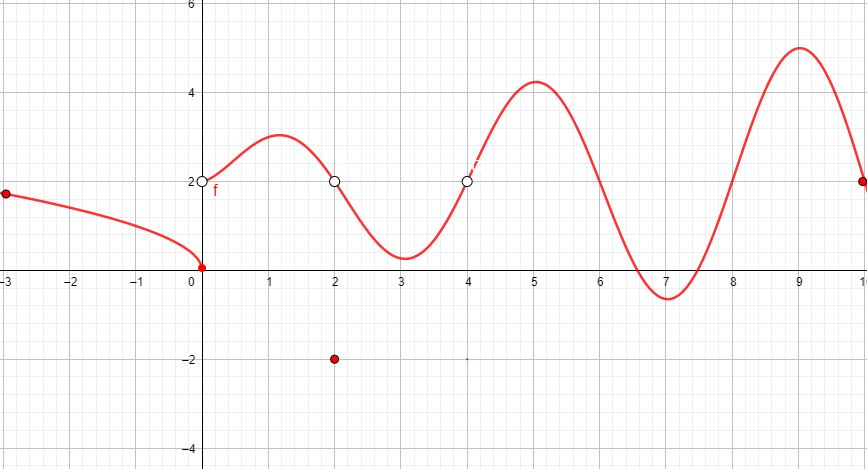
\includegraphics[scale=0.65]{problema_1.png}
    \label{fig:problema_1}
\end{figure}

\begin{soluciones}
    \subsubsection*{Solución}

    \begin{enumerate}[label=\alph*)]
        \item $\ds\lim_{x \rightarrow 2} f(x)=2$
        \item $\ds\lim_{x \rightarrow 4} f(x)=2$
        \item $\ds\lim_{x \rightarrow 0} f(x)=$ no existe ya que $\ds\lim_{x \rightarrow 0^{-}} f(x)=0 \neq \ds\lim_{x \rightarrow 0^{+}} f(x)=2$
    \end{enumerate}
\end{soluciones}

\subsection*{Problema 2}
Trace la gráfica de un ejemplo de una función $f$ que cumpla con todas las condiciones dadas.

\begin{enumerate}[label=\alph*)]
  \item $\ds\lim _{x \rightarrow-4^{+}} f(x)=-\infty$
  \item $\ds\lim _{x \rightarrow-4^{-}} f(x)=0$
  \item $\ds\lim _{x \rightarrow-2} f(x)=$ existe y $-2 \notin \operatorname{Dom}(f)$
  \item $\ds\lim _{x \rightarrow 0} f(x)=$ no existe
\end{enumerate}

\begin{soluciones}
  \subsubsection*{Solución}

  La gráfica de un ejemplo de función que cumple las condiciones dadas se muestra en la figura.

  \begin{figure}[H]
    \centering
    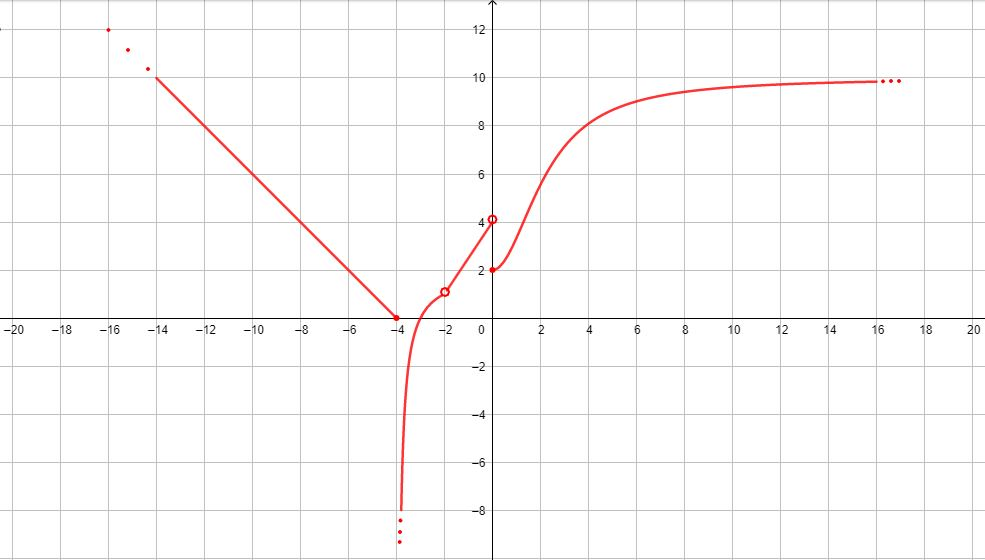
\includegraphics[scale=0.6]{solucion_2.png}
    \label{fig:solucion_2}
  \end{figure}
\end{soluciones}

\subsection*{Problema 3}
Para la función $f(x)=\dfrac{\sqrt{x}-\sqrt{2}}{|x-2|}$, responda las siguientes preguntas:

\begin{enumerate}[label=\alph*)]
  \item Determine el valor de $\ds\lim _{x \rightarrow 0^{+}} f(x)$.
  \item ¿Existe el $\ds\lim _{x \rightarrow 2} f(x)$? Justifique su respuesta. En caso afirmativo, ¿cuál es su valor?
\end{enumerate}

\begin{soluciones}
  \subsubsection*{Solución}

  Note que, el dominio de la función $f$ son los valores reales no negativos diferentes de 2 y que

  $$
  |x-2|=\left\{\begin{array}{lll}
  x-2 & \text { si } & x \geq 2 \\
  2-x & \text { si } & x<2
  \end{array}\right.
  $$
  
  entonces, la función $f$ puede escribirse como

  $$
  f(x)=\left\{\begin{array}{ccc}
  \dfrac{\sqrt{x}-\sqrt{2}}{2-x} & \text { si } & 0 \leq x<2 \\[15pt]
  \dfrac{\sqrt{x}-\sqrt{2}}{x-2} & \text { si } & x>2
  \end{array}\right.
  $$

  o, equivalentemente, como

  $$
  f(x)=\left\{\begin{array}{lcc}
  \dfrac{1}{-(\sqrt{x}+\sqrt{2})} & \text { si } & 0 \leq x<2 \\[15pt]
  \dfrac{1}{\sqrt{x}+\sqrt{2}} & \text { si } & x>2
  \end{array}\right.
  $$

  ya que

  $$
  2-x=(\sqrt{2}-\sqrt{x})(\sqrt{2}+\sqrt{x})=-(\sqrt{x}-\sqrt{2})(\sqrt{x}+\sqrt{2})
  $$

  y luego

  $$
  x-2=(\sqrt{x}-\sqrt{2})(\sqrt{x}+\sqrt{2})
  $$

  Así,

  $$
  \begin{aligned}
  \lim _{x \rightarrow 0^{+}} f(x) & =\lim _{x \rightarrow 0^{+}} \frac{1}{-(\sqrt{x}+\sqrt{2})} \\
  & =\frac{\lim _{x \rightarrow 0} 1}{-\left(\lim _{x \rightarrow 0^{+}} \sqrt{x}+\lim _{x \rightarrow 0} \sqrt{2}\right)} \\
  & =\frac{1}{-(0+\sqrt{2})} \\
  & =-\frac{1}{\sqrt{2}} \\
  & =-\frac{\sqrt{2}}{2}
  \end{aligned}
  $$

  Para la parte b) se estudian los límites laterales

  $$
  \begin{aligned}
  \lim _{x \rightarrow 2^{-}} f(x) & =\lim _{x \rightarrow 2^{-}} \frac{1}{-(\sqrt{x}+\sqrt{2})} \\
  & =\frac{\lim _{x \rightarrow 0} 1}{-\left(\lim _{x \rightarrow 2^{-}} \sqrt{x}+\lim _{x \rightarrow 2^{-}} \sqrt{2}\right)} \\
  & =\frac{1}{-(\sqrt{2}+\sqrt{2})} \\
  & =-\frac{1}{2 \sqrt{2}} \\
  & =-\frac{\sqrt{2}}{4}
  \end{aligned}
  $$

  $$
  \begin{aligned}
  \lim _{x \rightarrow 2^{+}} f(x) & =\lim _{x \rightarrow 2^{+}} \frac{1}{\sqrt{x}+\sqrt{2}} \\
  & =\frac{\lim _{x \rightarrow 0} 1}{\lim _{x \rightarrow 2^{+}} \sqrt{x}+\lim _{x \rightarrow 2^{+}} \sqrt{2}} \\
  & =\frac{1}{\sqrt{2}+\sqrt{2}} \\
  & =\frac{1}{2 \sqrt{2}} \\
  & =\frac{\sqrt{2}}{4}
  \end{aligned}
  $$

  Entonces, como $\lim _{x \rightarrow 2^{+}} f(x) \neq \lim _{x \rightarrow 2^{-}} f(x)$, el $\lim _{x \rightarrow 2} f(x)$ no existe.
\end{soluciones}

\subsection*{Problema 4}
Demuestre, usando la definición, que

$$\lim_{x \rightarrow-1} \frac{-5+3 x}{2}=-4
$$

\begin{soluciones}
  \subsubsection*{Solución}

  Sea $\varepsilon$ un número positivo dado. Se debe determinar un número positivo $\delta$ tal que:

  $$
  \text { si }|x-(-1)|<\delta \text { entonces }\left|\frac{-5+3 x}{2}-(-4)\right|<\varepsilon
  $$

  o, equivalentemente,

  $$
  \text { si }|x+1|<\delta \text { entonces }\left|\frac{-5+3 x}{2}+4\right|<\varepsilon
  $$

  Note que,

  $$
  \begin{aligned}
  \left|\frac{-5+3 x}{2}+4\right| & =\left|\frac{-5+3 x+8}{2}\right| \\
  & =\left|\frac{3 x+3}{2}\right| \\
  & =\left|\frac{3}{2}(x+1)\right| \\
  & =\frac{3}{2}|x+1|
  \end{aligned}
  $$

  y, si $|x+1|<\delta$, entonces $\frac{3}{2}|(x+1)|<\frac{3}{2} \delta$. Es decir, que:

  $$
  \text { si }|x+1|<\delta \text { entonces, }\left|\frac{-5+3 x}{2}+4\right|=\frac{3}{2}|x+1|<\frac{3}{2} \delta
  $$

  Así, para garantizar que $\left|\frac{-5+3 x}{2}+4\right|<\epsilon$, basta garantizar que $\frac{3}{2} \delta \leq \varepsilon$. En particular, basta considerar $\delta=\frac{2}{3} \varepsilon$. \medbreak

  Para la verificación, observe que, para $\varepsilon>0$ dado, si se toma $\delta=\frac{2}{3} \varepsilon$
  $$
  \begin{aligned}
  |x+1|<\delta & \Longrightarrow|x+1|<\frac{2}{3} \varepsilon \\
  & \Longrightarrow \frac{3}{2}|x+1|<\frac{3}{2} \frac{2}{3} \varepsilon \\
  & \Longrightarrow \underbrace{\frac{3}{2}|x+1|}_{\downarrow}<\varepsilon \\
  & \Longrightarrow\left|\frac{-5+3 x}{2}+4\right|<\varepsilon
  \end{aligned}
  $$
  lo cual demuestra lo requerido.
\end{soluciones}

\subsection*{Problema 5}
Determine, si corresponde, la ecuación de la(s) asíntota(s) vertical(es) de la función dada:

\begin{enumerate}[label=\alph*)]
  \item $f(x)=\dfrac{\sqrt{4 x^2+2020}}{3 x-6}$
  \item $f(x)=\dfrac{x^3-x}{x^2-6 x+5}$
  \item $f(x)=\dfrac{-2 e^x}{e^x-5}$
\end{enumerate}

\begin{soluciones}
  \subsubsection*{Solución}

  \begin{enumerate}[label=\alph*)]
    \item $f(x)=\dfrac{\sqrt{4 x^2+2020}}{3 x-6}$
    
    Note que el denominador de $f(x)$ es cero si $x=2$, por lo que la recta de ecuación $x=2$ es una posible asíntota vertical. El numerador es $\sqrt{2036}$, que es mayor que cero, y cuando $x$ tiende a 2 por la derecha $\left(2^{+}\right)$, la expresión $3 x-6$ toma valores positivos que tienden a cero. Entonces,

    $$
    \lim _{x \rightarrow 2^{+}} f(x)=\lim _{x \rightarrow 2^{+}} \frac{\sqrt{4 x^2+2020}}{3 x-6}=+\infty
    $$

    Así, la recta de ecuación $x=2$ es una asíntota vertical de $f$.
    Además, debido a que cuando $x$ tiende a 2 por la izquierda $\left(2^{-}\right)$, la expresión $3 x-6$ toma valores negativos que tienden a cero, se tiene que

    $$
    \lim _{x \rightarrow 2^{-}} f(x)=\lim _{x \rightarrow 2^{-}} \frac{\sqrt{4 x^2+2020}}{3 x-6}=-\infty
    $$

    lo cual, también indica que la recta de ecuación $x=2$ es una asíntota vertical de la función $f$.

    \item $f(x)=\dfrac{x^3-x}{x^2-6 x+5}$
    
    En este caso el denominador de la función racional dada se anula cuando $x=1$ y cuando $x=5$, por lo que las rectas de ecuación $x=1$ y $x=5$ son posibles asíntotas verticales.

    Sin embargo, para el caso en el que $x=1$, se tiene que

    $$
    \begin{aligned}
    \lim _{x \rightarrow 1} f(x) & =\lim _{x \rightarrow 1} \frac{x(x-1)(x+1)}{(x-1)(x-5)} \\
    & =\lim _{x \rightarrow 1} \frac{(x-1)}{x-1} \frac{x(x+1)}{(x-5)} \\
    & =\lim _{x \rightarrow 1} \frac{(x-1)}{(x-1)} \lim _{x \rightarrow 1} \frac{x(x+1)}{(x-5)} \\
    & =1 \cdot\left(\frac{2}{-4}\right) \\
    & =-\frac{1}{2}
    \end{aligned}
    $$

    es decir, el límite es finito, por lo que la recta de ecuación $x=1$ no corresponde a una asíntota vertical de la función $f$.

    Para el caso de $x=5$,

    $$
    \begin{aligned}
    \lim _{x \rightarrow 5^{+}} f(x) & =\lim _{x \rightarrow 5^{+}} \frac{x(x-1)(x+1)}{(x-1)(x-5)} \\
    & =\lim _{x \rightarrow 5^{+}} \frac{(x-1)}{(x-1)} \lim _{x \rightarrow 5^{+}} \frac{x(x+1)}{x-5} \\
    & =1 \cdot \lim _{x \rightarrow 5^{+}} \frac{x(x+1)}{(x-5)} \\
    & =\lim _{x \rightarrow 5^{+}} \frac{x(x+1)}{(x-5)} \\
    & =\infty
    \end{aligned}
    $$

    ya que cuando $x$ tiende a 5 por la derecha $\left(5^{+}\right)$, la expresión $x(x+1)$ tiende a 30 , que es mayor que cero, y la expresión $x-5$ toma valores positivos que tienden cero. Entonces, la recta de ecuación $x=5$ es una asíntota vertical de $f(x)$.

    También, observe que

    $$
    \begin{aligned}
    \lim _{x \rightarrow 5^{-}} f(x) & =\lim _{x \rightarrow 5^{-}} \frac{x(x-1)(x+1)}{(x-1)(x-5)} \\
    & =\lim _{x \rightarrow 5^{+}} \frac{(x-1)}{(x-1)} \lim _{x \rightarrow 5^{+}} \frac{x(x+1)}{x-5} \\
    & =1 \cdot \lim _{x \rightarrow 5^{-}} \frac{x(x+1)}{(x-5)} \\
    & =\lim _{x \rightarrow 5^{-}} \frac{x(x+1)}{(x-5)} \\
    & =-\infty
    \end{aligned}
    $$

    ya que cuando $x$ tiende a 5 por la izquierda ($5^-$), la expresión $x(x+1)$ tiende a 30 , que es mayor que cero, y la expresión $x-5$ toma valores negativos que tienden cero.
    El hecho de que el $\lim _{x \rightarrow 5^{-}} f(x)=-\infty$ también indica que la recta de ecuación $x=5$ es una asíntota vertical de $f$.

    \item $f(x)=\dfrac{-2 e^x}{e^x-5}$
    
    Para esta función el denominador de $f(x)$ es cero si $x=\ln (5)$. El numerador es $-2 e^{\ln (5)}=-2 \cdot 5=-10$, que es menor que cero, entonces,

    $$
    \lim _{x \rightarrow\left((\ln (5))^{+}\right.} f(x)=\lim _{x \rightarrow\left((\ln (5))^{+}\right.} \frac{-2 e^x}{e^x-5}=-\infty
    $$

    ya que cuando $x$ tiende a $\ln (5)$ por la derecha $\left((\ln (5))^{+}\right)$, la expresión $e^x-5$ toma valores positivos que tienden a cero. Así, la recta de ecuacón $x=\ln (5)$ es una asíntota vertical de $f$.
    Además,

    $$
    \lim _{x \rightarrow\left((\ln (5))^{-}\right.} f(x)=\lim _{x \rightarrow\left((\ln (5))^{-}\right.} \frac{-2 e^x}{e^x-5}=\infty
    $$

    ello debido a que cuando $x$ tiende a $\ln (5)$ por la izquierda $\left((\ln (5))^{-}\right)$, la expresión $e^x-5$ toma valores negativos que tienden a cero. Esto también indica que $x=\ln (5)$ es una asíntota vertical de $f$.
  \end{enumerate}
\end{soluciones}

\subsection*{Problema 6}
Estudie si cada uno de los límites indicados existe o no. Si existe, determine su valor, en caso contrario, explique por qué:

\begin{enumerate}[label=\alph*)]
  \item $\ds\lim _{x \rightarrow 4} \dfrac{5-\sqrt{9+x^2}}{1-\sqrt{5-x}}$
  \item $\ds\lim _{x \rightarrow 0} \dfrac{x}{\sqrt[3]{x-27}+3}$
\end{enumerate}

\begin{soluciones}
  \subsubsection*{Solución}

  \begin{enumerate}[label=\alph*)]
    \item $\ds\lim _{x \rightarrow 4} \dfrac{5-\sqrt{9+x^2}}{1-\sqrt{5-x}}$
    
    Note que no se puede determinar el límite por sustitución porque si $f(x)=\dfrac{5-\sqrt{9+x^2}}{1-\sqrt{5-x}}, f(4)$ no está definida. Para calcularlo se realizan, previamente, varias operaciones algebraicas.

    $$
    \begin{aligned}
    \lim _{x \rightarrow 4} \frac{5-\sqrt{9+x^2}}{1-\sqrt{5-x}} & =\lim _{x \rightarrow 4} \frac{\left(5-\sqrt{9+x^2}\right)\left(5+\sqrt{9+x^2}\right)(1+\sqrt{5-x})}{(1-\sqrt{5-x})(1+\sqrt{5-x})\left(5+\sqrt{9+x^2}\right)} \\
    & =\lim _{x \rightarrow 4} \frac{\left(16-x^2\right)}{(x-4)} \lim _{x \rightarrow 4} \frac{(1+\sqrt{5-x})}{\left(5+\sqrt{9+x^2}\right)} \\
    & =\lim _{x \rightarrow 4} \frac{(4-x)(4+x)}{(x-4)} \lim _{x \rightarrow 4} \frac{(1+\sqrt{5-x})}{\left(5+\sqrt{9+x^2}\right)} \\
    & =\lim _{x \rightarrow 4} \frac{(4-x)}{(x-4)} \lim _{x \rightarrow 4}(4+x) \lim _{x \rightarrow 4} \frac{(1+\sqrt{5-x})}{\left(5+\sqrt{9+x^2}\right)} \\
    & =(-1) 8 \frac{2}{10} \\
    & =-\frac{8}{5}
    \end{aligned}
    $$

    \item $\ds\lim _{x \rightarrow 0} \dfrac{x}{\sqrt[3]{x-27}+3}$
    
    Al considerar $f(x)=\dfrac{x}{\sqrt[3]{x-27}+3}, f(0)$ no está definida, por lo tanto, no se puede determinar el límite por sustitución. Para calcularlo se realizan, previamente, varias operaciones algebraicas.

    $$
    \begin{aligned}
    \lim _{x \rightarrow 0} \frac{x}{\sqrt[3]{x-27}+3} & =\lim _{x \rightarrow 0} \frac{x\left((\sqrt[3]{x-27})^2-3 \sqrt[3]{x-27}+3^2\right)}{(\sqrt[3]{x-27}+3)\left((\sqrt[3]{x-27})^2-3 \sqrt[3]{x-27}+3^2\right)} \\
    & =\lim _{x \rightarrow 0} \frac{x\left((\sqrt[3]{x-27})^2-3 \sqrt[3]{x-27}+9\right)}{(\sqrt[3]{x-27})^3+3^3} \\
    & =\lim _{x \rightarrow 0} \frac{x\left((\sqrt[3]{x-27})^2-3 \sqrt[3]{x-27}+9\right)}{x} \\
    & =\lim _{x \rightarrow 0} \frac{x}{x} \lim _{x \rightarrow 0}\left((\sqrt[3]{x-27})^2-3 \sqrt[3]{x-27}+9\right) \\
    & =1 \cdot\left((-3)^2-3(-3)+9\right) \\
    & =27
    \end{aligned}
    $$
  \end{enumerate}
\end{soluciones}

\newpage

% Evaluación de la ayudantía
\subsection*{Evaluación de la ayudantía}
\noindent Les invito a responder una breve encuesta para evaluar el desempeño en la ayudantía de hoy, con la finalidad de mejorar en las siguientes. Puedes escanear el código QR o hacer click \href{https://forms.office.com/r/0JwNEUVYjd}{acá}.

\begin{figure}[H]
    \centering
    
\includegraphics[height=5.5cm]{qr.png}
    % \caption{Código QR de evaluación de la ayudantía}
    \label{fig:qr}
\end{figure}

% Para generar un código QR que redirija a un sitio web de interés, como una encuesta de evaluación, se pueden encontrar distintas herramientas online. En mi caso particular, para generar este código utilicé https://www.qr-code-generator.com/

\end{document}